Race time}\label{result_racetime}
We posited that strategy choice would greatly impact race time in the slalom course. By enabling the reinforcement learning group to directly evaluate strategies through observing times, we expected that they would learn to select better strategies and consequently perform better over the course of the sessions compared to the two supervised learning groups. As a first step in the analysis, we assessed whether there were pure time differences between the groups across the different sessions without taking the chosen strategy into account.

\subsubsection{Greater improvement during acquisition with reinforcement learning than supervised (free choice) learning}\label{result_racetime_acquisition}
During the acquisition sessions, our hypothesis was that the skiers exposed to reinforcement learning would show greater race time improvement across the Free Choice 1 and Free Choice 2 sessions compared to the skiers in the supervised learning groups due to the direct evaluation of the strategies. Fig. \ref{fig: racetime}a presents mean race time estimates for treatment groups during the three acquisition sessions.

In the first acquisition session (Forced Exploration), we did not expect significant differences between the groups since all groups had the same number of trials on each strategy. Indeed, we found that the average race times did not significantly differ between reinforcement learning and supervised (free choice) learning. Indeed, we found that the average race times did not significantly differ between reinforcement learning and supervised (free choice) learning ($\beta$ = 0.06 , 95\% CI [-0.2, 0.32], $t$(92.727) = 0.48, $p$ = 0.631) and supervised (target skill) learning ($\beta$ = 0.18, 95\% CI[-0.08, 0.44], $t$(92.663) = 1.37, $p$ = 0.174). 

Group differences in race time improvement were by contrast expected during the next two acquisition sessions (Free Choice 1 and Free Choice 2), when the skiers or the coach had the autonomy to pick strategy. We found that all treatment groups significantly improved their race times from Forced Exploration to Free Choice 1 (Reinforcement learning: $\beta$ = -0.38, 95\% CI[-0.45, -0.31], $t$(91.632) = -10.82, $p$ $<$ 0.001; Supervised (free choice): $\beta$ = -0.3, 95\% CI[-0.37, -0.23], $t$(93.472) = -8.96, $p$ $<$ 0.001; Supervised (target skill): $\beta$ = -0.5, 95\% CI[-0.57, -0.44], $t$(91.95) = -15.08, $p$ $<$ 0.001). However, this improvement was significantly greater for supervised (target skill) learning, with coaches selecting the best theoretical strategy, than for reinforcement learning ($\beta$ = -0.12, 95\% CI[-0.22, -0.03], $t$(91.777) = -2.58, $p$ = 0.012).  In contrast, supervised (free choice) learning, where coaches made strategy choices for the skiers, improved less from Forced Exploration to Free Choice 1 than reinforcement learning, but this difference was not statistically significant ($\beta$ = 0.08, 95\% CI[-0.02, 0.17], $t$(92.5) = 1.61, $p$ = 0.110).

The improvement from Forced Exploration persisted for all groups in Free Choice 2 (Reinforcement learning: $\beta$ = -0.45, 95\% CI[-0.54, -0.36], $t$(95.164) = -9.99, $p$ $<$ 0.001; Supervised (free choice): $\beta$ = -0.31, 95\% CI[-0.39, -0.22], $t$(96.389) = -7.17, $p$ $<$ 0.001; Supervised (target skill): $\beta$ = -0.43, 95\% CI[-0.52, -0.35], $t$(96.196) = -10.07, $p$ $<$ 0.001). Descriptively, the average race time for the reinforcement learning group continued to improve from Free Choice 1 to Free Choice 2,  but plateaued for supervised (free choice) learning, resulting in a significant difference in change between the groups ($\beta$ = 0.14, 95\% CI[0.02, 0.26], $t$(95.743) = 2.26, $p$ = 0.026). In contrast, the supervised (target skill) learning group's race times declined from Free Choice 1 to Free Choice 2 such that their initial greater improvement in race time  
attenuated, resulting in a non-significant interaction effect ($\beta$ = 0.02, 95\% CI[-0.11, 0.14], $t$(95.651) = 0.26, $p$ = 0.798).

We did not, however, find statistical evidence that reinforcement learning performed better than supervised (free choice) or supervised (target skill) learning at Free Choice 1 or Free Choice 2 (Supplementary Table \ref{suptable_racetime_groupdiffeachsession}). Overall, this suggests that the three learning groups had varied learning trajectories across the three acquisition sessions, with the differing development seeming to be associated with the selection of strategies. 











Thus far, we have presented evidence that reinforcement learning improved more during the three acquisition sessions and performed better than supervised (free choice) learning during retention. Although reinforcement learning performed descriptively better than supervised (target skill) learning during acquisition and retention, this difference was not statistically significant. Our study was designed to examine whether the choice of strategies could account for the variation in time differences, with our hypothesis being that reinforcement learning learned to choose better strategies than supervised learning groups because they were able to learn the values of the strategies by directly observing the race times. To address this, we examined whether reinforcement learning learned to choose the theoretically best strategy and the individual skier's estimated best strategy more frequently than supervised (free choice) learning. Fig.\ref{fig: choice_descriptives} displays the percentage selections of the four strategies across all sessions.


No evidence that reinforcement learning chose the theoretical best strategy more often than supervised (free choice) learning}\label{result_strategychoice_theorybest}

We first tested whether reinforcement learning was more likely to choose the theoretical best strategy. The figure \ref{fig: choice_estimated} displays the predicted probabilities for the treatment groups across the sessions. 


\begin{figure}[H]
\centering
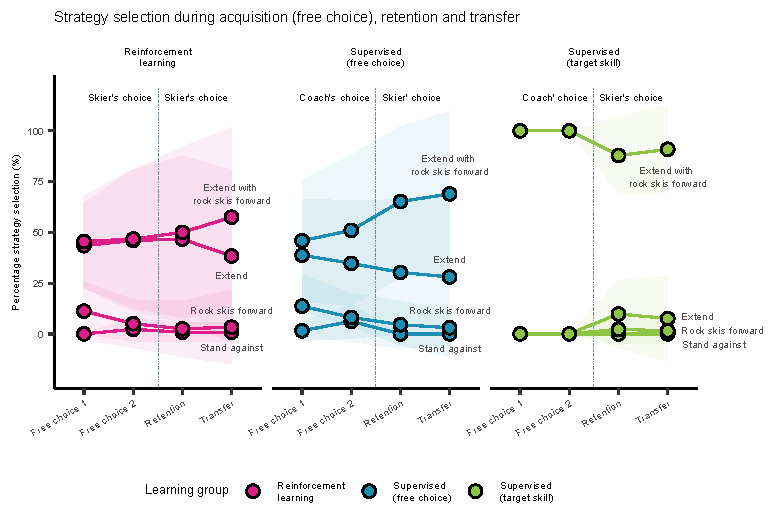
\includegraphics{figures/figure_choice_descriptivecount_4.pdf}
\caption{Strategy choices for skiers in each session, with bars indicating percentages and the numbers to the right of the bars showing the total count for
each strategy. Data has been aggregated from our multi-level structure for clarity}\label{fig: choice_descriptives}
\end{figure}

In the first acquisition session where the skier or coach were free to select strategy (Free Choice 1), neither reinforcement learning (0.43) nor supervised (free choice) learning (0.42) preferred the theoretically optimal strategy. This predicted probability difference was not significant ($\beta$ = 0.01, 95\% CI[-0.24, 0.27], $z$ = 0.11, $p$ = 0.912). 

Both groups remained conservative in their strategy selection during Free Choice 2: The reinforcement learning group increased its predicted probability marginally from 0.43 in Free Choice 1 to 0.45 in Free Choice 2, with no statistical significance ($\beta$ = 0.02, 95\% CI[-0.11, 0.14], $z$ = 0.26, $p$ = 0.791). Similarly, the supervised (free choice) learning group saw a slight increase from 0.43 in Free choice 1 to 0.5 in Free Choice 2, and this change was also not statistically significant ($\beta$ = 0.08, 95\% CI[-0.04, 0.21], $z$ = 1.32, $p$ = 0.188). The difference in change between groups was not statistically significant ($\beta$ = 0.07, 95\% CI[-0.11, 0.24], $z$ = 0.74, $p$ = 0.458) nor was the group difference at Free Choice 2 ($\beta$ = -0.05, 95\% CI[-0.31, 0.2], $z$ = -0.4, $p$ = 0.693). 

A noticeable trend emerged in retention, with skiers in supervised (free choice) learning also having the autonomy to independently select strategies, free from the coach's guidance. Here, supervised (free choice) learning significantly increased its predicted probability of selecting the theoretical best strategy, rising from 0.43 in Free Choice 2 to 0.45 in Retention ($\beta$ = 0.23, 95\% CI[0.09, 0.36], $z$ = 3.31, $p$ < 0.001). In the same transition, the change from 0.45 to 0.5 for the reinforcement learning group was not statistically significant ($\beta$ = 0.05, 95\% CI [-0.09, 0.19], $z$ = 0.72, $p$ = 0.469). The difference in change between the groups was not statistically significant ($\beta$ = 0.17, 95\% CI[-0.02,  0.37], $z$ = 1.74, $p$ = 0.081), nor was their difference at retention ($\beta$ = -0.23, 95\% CI[-0.48, 0.03], $z$ = -1.75, $p$ = 0.079).

The predicted probability of choosing the theoretical best strategy further increased for both groups in Transfer, but this increase was not statistically significant for reinforcement learning ($\beta$ = 0.11 , 95\% CI [ -0.04 ,  0.27 ], $z$ = 1.42 , $p$  =  0.155) or supervised (free choice) learning ($\beta$ = 0.05, 95\% CI[-0.07, 0.18], $z$ = 0.85, $p$ = 0.396). Neither their difference in change from retention ($\beta$ = -0.06, 95\% CI[-0.25, 0.14], $z$ = -0.58, $p$  =  0.564), nor the differences between the groups on transfer were significant ($\beta$ = -0.17, 95\% CI [-0.4, 0.07], $z$ = -1.41, $p$ = 0.159).


\begin{figure}[H]
\centering
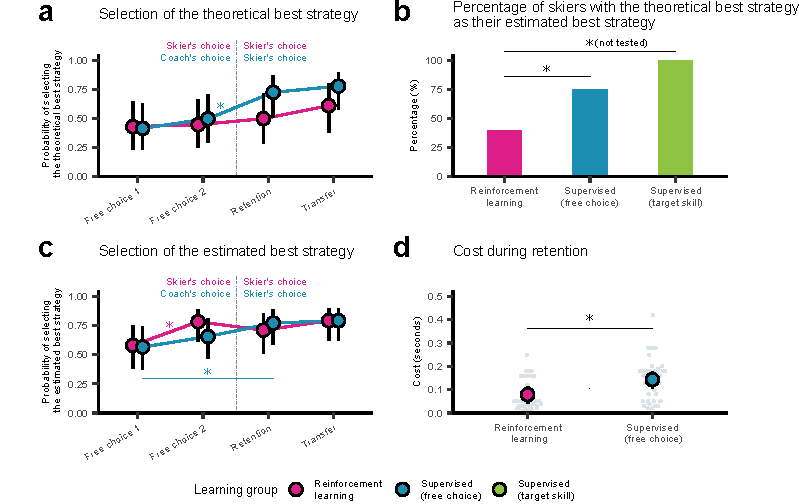
\includegraphics{figures/figure_choice_estimated_4.pdf}
\caption{Strategy selection for reinforcement learning (red) and supervised (free choice) learning (blue) during acquisition. \textbf{a.} Displays the estimated probability of choosing the theoretically best strategy (that is, extend with rocking skis forward) for both reinforcement learning and supervised (free choice) learning. \textbf{b.} Presents the estimated probability of selecting the empirically determined best strategy (that is, estimated using the sampling average method for each skier in the dataset). Intervals represent the 95\% confidence interval derived from the models. Asterisks (*) indicate a statistically significant interaction effect.}\label{fig: choice_estimated}
\end{figure}

\subsection{A higher proportion of skiers in the supervised (free choice) learning had the theoretical best strategy as their estimated best}\label{result_strategychoice_proportion}
We did not find evidence that the predicted probability of choosing the theoretical best strategy was higher on average among skiers in the reinforcement learning group compared to those in the supervised (free choice) learning group. In contrast, it was the supervised (free choice) learning group that increased their selection of this strategy. As a follow-up analysis, we investigated whether a higher proportion of skiers in the supervised (free choice) learning group had the theoretically best strategy as their estimated best strategy. Such a trend could suggest that the feedback from coaches during the learning attempts may have made this strategy more effective. 

Figure \ref{fig: choice_estimated}b shows the proportion of skiers for each group that had the theoretical best strategy as their estimated best strategy. In this analysis, we found that 40\% of skiers in reinforcement learning had the theoretically best strategy as their estimated best strategy compared to 75\% in the supervised (free choice) group. A chi-square test revealed a statistical significant association between groups $\chi^2$ = 6.42, $p$ = 0.01). Because all skiers in the supervised (target skill) group had the theoretical best as their estimated best strategy, we did not include this group in this test.  


\subsubsection{No convincing evidence that reinforcement learning selected the individual skier's estimated best strategy more often}\label{result_strategychoice_estbest}
The observation that skiers in supervised (free choice) learning increasingly opted for the theoretically best strategy more across sessions than those in reinforcement learning does not necessarily imply a more frequent selection of their estimated best strategy. Consequently, we investigated whether reinforcement learning resulted in a higher predicted probability of selecting the estimated best strategy. Figure \ref{fig: choice_estimated}c displays the predicted probabilities of choosing the estimated best strategy for the treatment groups across the sessions. 

In free choice 1, the predicted probability difference between reinforcement learning (0.58) and supervised (free choice) learning (0.57) was small and not significant ($\beta$ = 0.01, 95\% CI [-0.22, 0.24], $z$ = 0.12, $p$ = 0.904). 

In free choice 2, the predicted probability of choosing the estimated best strategy significantly increased for the reinforcement learning group ($\beta$ = 0.2, 95\% CI [0.09, 0.32], $z$ = 3.39, $p$  $<$ 0.001), but not for the supervised (free choice) learning group ($\beta$ = 0.09, 95\% CI [-0.03, 0.21], $z$ = 1.48, $p$ = 0.140). Their difference in change was not significant, however ($\beta$ = -0.11, 95\% CI [-0.28, 0.05], $z$ = -1.33, $p$ = 0.184), nor was their predicted probability difference at free choice 3 ($\beta$ = 0.13, 95\% CI [-0.06, 0.32 ], $z$ = 1.3 , $p$  =  0.194).

When skiers in the supervised (free choice) learning group were given the freedom to choose strategies on retention, their predicted probabilities of choosing their estimated best strategy also increased, although this increase was not statistically significant ($\beta$ = 0.12, 95\% CI [0, 0.24], $z$ = 1.88, $p$ = 0.060). This was in contrast to the reinforcement learning group, where the predicted probability decreased by 0.07 from free choice 2 to retention, but this also was not statistically significant ($\beta$ = -0.07, 95\% CI [-0.19, 0.04], $z$ = -1.25, $p$ = 0.213). However, their difference in change was statistically significant ($\beta$ = 0.19, 95\% CI [0.02, 0.36], $z$ = 2.2, $p$ = 0.028). We did, however,  not find any statistically significant difference between the groups at retention ($\beta$ = -0.06, 95\% CI[-0.26, 0.14], $z$ = -0.61, $p$ = 0.544).

Neither reinforcement learning ($\beta$ = 0.08, 95\% CI[-0.04, 0.2], $z$ = 1.31, $p$ = 0.190) nor supervised (free choice) learning ($\beta$ = 0.02, 95\% CI[-0.09, 0.13], $z$ = 0.35, $p$ = 0.727) showed a significant increase in predicted probabilities from the retention phase to the transfer phase. This difference in change was not significant ($\beta$ = -0.06 , 95\% CI [-0.23, 0.1], $z$ = -0.73, $p$ = 0.467), nor was the predicted probability difference at transfer ($\beta$ = 0, 95\% CI [-0.17, 0.17], $z$ = 0, $p$ = 0.999).

\subsubsection{Reinforcement learning had a lower costs when performing suboptimal strategies compared to  reinforcement learning}\label{subsubsec3}
Choosing the estimated best strategy is one thing, but avoiding the selection of a strategy significantly worse than the estimated best strategy is another. In a follow-up analysis, we computed the expected difference between the skiers' chosen suboptimal strategy and their estimated best strategy, which we referred to as 'cost.' A lower cost implies that the performer has better grasped the effects of various strategies. This analysis revealed that reinforcement learning had lower costs than supervised (free choice) learning did  ($\beta$ = 0.06 , 95\% CI [ 0.01 ,  0.12 ], $t$( 30.789 ) = 2.55 , $p$  =  0.016), suggesting that they had better learned the strategies.

\subsubsection{Large win-stay, lose-switch signatures but no convincing evidence for difference between groups}\label{wsls}
To test the extent to which coaches in supervised (free choice) learning and skiers in reinforcement learning utilized trial feedback to make decisions, we conducted a 'win-stay, lose-switch' (WSLS) analysis. In this analysis, heightened sensitivity is indicated by a high predicted probability of repeating an action following good feedback and a low predicted probability following bad feedback on a previous trial.

Figure \ref{fig: choice_wsls} shows the predicted probability of repeating the strategy on the previous trial if the feedback was good. We found statistically significant estimated marginal effects at the mean (MEM) for both reinforcement learning  ($\beta$ = -0.18, 95\% CI[-0.26, -0.11], $z$ = -4.8,$p$ < 0.001) and supervised (free choice) learning ($\beta$ = -0.11 , 95\% CI [ -0.17 ,  -0.04 ], $z$ = -3.29 , $p$  <  0.001). These findings suggest that both groups had a higher predicted probability of repeating a strategy if the previous trial feedback was good. Despite the large descriptive difference in the marginal effect between groups, this difference was not statistically  significant ($\beta$ = -0.08, 95\% CI [-0.17, 0.02], $z$ = -1.55, $p$ $=$ 0.121).




\begin{figure}[H]
\centering
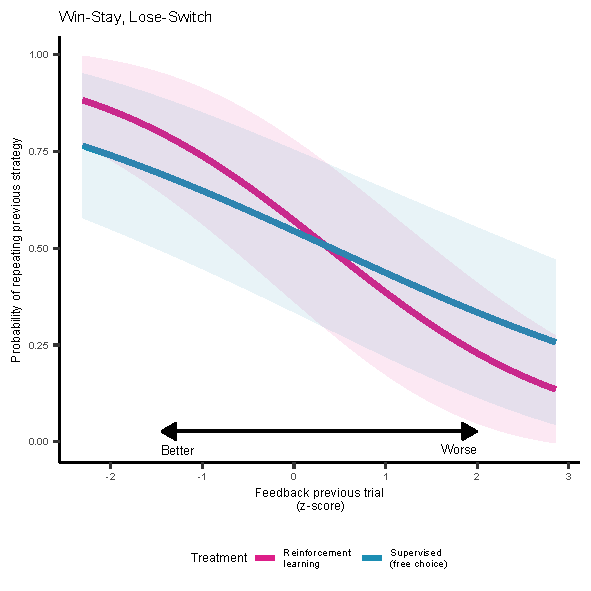
\includegraphics{figures/figure_winstaylooseshift.pdf}
\caption{Win-stay, lose-switch comparison between reinforcement learning and supervised (free choice) learning. The line shows the predicted probability of repeating the previously chosen strategy based on its trial feedback, along with a 95\%CI in the ribbon. In this model, higher or lower probabilities with better and worse feedback mean greater sensitivity to feedback}\label{fig: choice_wsls}
\end{figure}

